% Generated by Sphinx.
\def\sphinxdocclass{report}
\documentclass[letterpaper,10pt,spanish]{sphinxmanual}
\usepackage[utf8]{inputenc}
\DeclareUnicodeCharacter{00A0}{\nobreakspace}
\usepackage{cmap}
\usepackage[T1]{fontenc}
\usepackage{babel}
\usepackage{times}
\usepackage[Sonny]{fncychap}
\usepackage{longtable}
\usepackage{sphinx}
\usepackage{multirow}

\addto\captionsspanish{\renewcommand{\figurename}{Figura }}
\addto\captionsspanish{\renewcommand{\tablename}{Tabla }}
\floatname{literal-block}{Lista }



\title{quick2wire-ingeniería Documentation}
\date{09 de July de 2015}
\release{1}
\author{Diego Martín}
\newcommand{\sphinxlogo}{}
\renewcommand{\releasename}{Publicación}
\makeindex

\makeatletter
\def\PYG@reset{\let\PYG@it=\relax \let\PYG@bf=\relax%
    \let\PYG@ul=\relax \let\PYG@tc=\relax%
    \let\PYG@bc=\relax \let\PYG@ff=\relax}
\def\PYG@tok#1{\csname PYG@tok@#1\endcsname}
\def\PYG@toks#1+{\ifx\relax#1\empty\else%
    \PYG@tok{#1}\expandafter\PYG@toks\fi}
\def\PYG@do#1{\PYG@bc{\PYG@tc{\PYG@ul{%
    \PYG@it{\PYG@bf{\PYG@ff{#1}}}}}}}
\def\PYG#1#2{\PYG@reset\PYG@toks#1+\relax+\PYG@do{#2}}

\expandafter\def\csname PYG@tok@gd\endcsname{\def\PYG@tc##1{\textcolor[rgb]{0.63,0.00,0.00}{##1}}}
\expandafter\def\csname PYG@tok@gu\endcsname{\let\PYG@bf=\textbf\def\PYG@tc##1{\textcolor[rgb]{0.50,0.00,0.50}{##1}}}
\expandafter\def\csname PYG@tok@gt\endcsname{\def\PYG@tc##1{\textcolor[rgb]{0.00,0.27,0.87}{##1}}}
\expandafter\def\csname PYG@tok@gs\endcsname{\let\PYG@bf=\textbf}
\expandafter\def\csname PYG@tok@gr\endcsname{\def\PYG@tc##1{\textcolor[rgb]{1.00,0.00,0.00}{##1}}}
\expandafter\def\csname PYG@tok@cm\endcsname{\let\PYG@it=\textit\def\PYG@tc##1{\textcolor[rgb]{0.25,0.50,0.56}{##1}}}
\expandafter\def\csname PYG@tok@vg\endcsname{\def\PYG@tc##1{\textcolor[rgb]{0.73,0.38,0.84}{##1}}}
\expandafter\def\csname PYG@tok@m\endcsname{\def\PYG@tc##1{\textcolor[rgb]{0.13,0.50,0.31}{##1}}}
\expandafter\def\csname PYG@tok@mh\endcsname{\def\PYG@tc##1{\textcolor[rgb]{0.13,0.50,0.31}{##1}}}
\expandafter\def\csname PYG@tok@cs\endcsname{\def\PYG@tc##1{\textcolor[rgb]{0.25,0.50,0.56}{##1}}\def\PYG@bc##1{\setlength{\fboxsep}{0pt}\colorbox[rgb]{1.00,0.94,0.94}{\strut ##1}}}
\expandafter\def\csname PYG@tok@ge\endcsname{\let\PYG@it=\textit}
\expandafter\def\csname PYG@tok@vc\endcsname{\def\PYG@tc##1{\textcolor[rgb]{0.73,0.38,0.84}{##1}}}
\expandafter\def\csname PYG@tok@il\endcsname{\def\PYG@tc##1{\textcolor[rgb]{0.13,0.50,0.31}{##1}}}
\expandafter\def\csname PYG@tok@go\endcsname{\def\PYG@tc##1{\textcolor[rgb]{0.20,0.20,0.20}{##1}}}
\expandafter\def\csname PYG@tok@cp\endcsname{\def\PYG@tc##1{\textcolor[rgb]{0.00,0.44,0.13}{##1}}}
\expandafter\def\csname PYG@tok@gi\endcsname{\def\PYG@tc##1{\textcolor[rgb]{0.00,0.63,0.00}{##1}}}
\expandafter\def\csname PYG@tok@gh\endcsname{\let\PYG@bf=\textbf\def\PYG@tc##1{\textcolor[rgb]{0.00,0.00,0.50}{##1}}}
\expandafter\def\csname PYG@tok@ni\endcsname{\let\PYG@bf=\textbf\def\PYG@tc##1{\textcolor[rgb]{0.84,0.33,0.22}{##1}}}
\expandafter\def\csname PYG@tok@nl\endcsname{\let\PYG@bf=\textbf\def\PYG@tc##1{\textcolor[rgb]{0.00,0.13,0.44}{##1}}}
\expandafter\def\csname PYG@tok@nn\endcsname{\let\PYG@bf=\textbf\def\PYG@tc##1{\textcolor[rgb]{0.05,0.52,0.71}{##1}}}
\expandafter\def\csname PYG@tok@no\endcsname{\def\PYG@tc##1{\textcolor[rgb]{0.38,0.68,0.84}{##1}}}
\expandafter\def\csname PYG@tok@na\endcsname{\def\PYG@tc##1{\textcolor[rgb]{0.25,0.44,0.63}{##1}}}
\expandafter\def\csname PYG@tok@nb\endcsname{\def\PYG@tc##1{\textcolor[rgb]{0.00,0.44,0.13}{##1}}}
\expandafter\def\csname PYG@tok@nc\endcsname{\let\PYG@bf=\textbf\def\PYG@tc##1{\textcolor[rgb]{0.05,0.52,0.71}{##1}}}
\expandafter\def\csname PYG@tok@nd\endcsname{\let\PYG@bf=\textbf\def\PYG@tc##1{\textcolor[rgb]{0.33,0.33,0.33}{##1}}}
\expandafter\def\csname PYG@tok@ne\endcsname{\def\PYG@tc##1{\textcolor[rgb]{0.00,0.44,0.13}{##1}}}
\expandafter\def\csname PYG@tok@nf\endcsname{\def\PYG@tc##1{\textcolor[rgb]{0.02,0.16,0.49}{##1}}}
\expandafter\def\csname PYG@tok@si\endcsname{\let\PYG@it=\textit\def\PYG@tc##1{\textcolor[rgb]{0.44,0.63,0.82}{##1}}}
\expandafter\def\csname PYG@tok@s2\endcsname{\def\PYG@tc##1{\textcolor[rgb]{0.25,0.44,0.63}{##1}}}
\expandafter\def\csname PYG@tok@vi\endcsname{\def\PYG@tc##1{\textcolor[rgb]{0.73,0.38,0.84}{##1}}}
\expandafter\def\csname PYG@tok@nt\endcsname{\let\PYG@bf=\textbf\def\PYG@tc##1{\textcolor[rgb]{0.02,0.16,0.45}{##1}}}
\expandafter\def\csname PYG@tok@nv\endcsname{\def\PYG@tc##1{\textcolor[rgb]{0.73,0.38,0.84}{##1}}}
\expandafter\def\csname PYG@tok@s1\endcsname{\def\PYG@tc##1{\textcolor[rgb]{0.25,0.44,0.63}{##1}}}
\expandafter\def\csname PYG@tok@gp\endcsname{\let\PYG@bf=\textbf\def\PYG@tc##1{\textcolor[rgb]{0.78,0.36,0.04}{##1}}}
\expandafter\def\csname PYG@tok@sh\endcsname{\def\PYG@tc##1{\textcolor[rgb]{0.25,0.44,0.63}{##1}}}
\expandafter\def\csname PYG@tok@ow\endcsname{\let\PYG@bf=\textbf\def\PYG@tc##1{\textcolor[rgb]{0.00,0.44,0.13}{##1}}}
\expandafter\def\csname PYG@tok@sx\endcsname{\def\PYG@tc##1{\textcolor[rgb]{0.78,0.36,0.04}{##1}}}
\expandafter\def\csname PYG@tok@bp\endcsname{\def\PYG@tc##1{\textcolor[rgb]{0.00,0.44,0.13}{##1}}}
\expandafter\def\csname PYG@tok@c1\endcsname{\let\PYG@it=\textit\def\PYG@tc##1{\textcolor[rgb]{0.25,0.50,0.56}{##1}}}
\expandafter\def\csname PYG@tok@kc\endcsname{\let\PYG@bf=\textbf\def\PYG@tc##1{\textcolor[rgb]{0.00,0.44,0.13}{##1}}}
\expandafter\def\csname PYG@tok@c\endcsname{\let\PYG@it=\textit\def\PYG@tc##1{\textcolor[rgb]{0.25,0.50,0.56}{##1}}}
\expandafter\def\csname PYG@tok@mf\endcsname{\def\PYG@tc##1{\textcolor[rgb]{0.13,0.50,0.31}{##1}}}
\expandafter\def\csname PYG@tok@err\endcsname{\def\PYG@bc##1{\setlength{\fboxsep}{0pt}\fcolorbox[rgb]{1.00,0.00,0.00}{1,1,1}{\strut ##1}}}
\expandafter\def\csname PYG@tok@mb\endcsname{\def\PYG@tc##1{\textcolor[rgb]{0.13,0.50,0.31}{##1}}}
\expandafter\def\csname PYG@tok@ss\endcsname{\def\PYG@tc##1{\textcolor[rgb]{0.32,0.47,0.09}{##1}}}
\expandafter\def\csname PYG@tok@sr\endcsname{\def\PYG@tc##1{\textcolor[rgb]{0.14,0.33,0.53}{##1}}}
\expandafter\def\csname PYG@tok@mo\endcsname{\def\PYG@tc##1{\textcolor[rgb]{0.13,0.50,0.31}{##1}}}
\expandafter\def\csname PYG@tok@kd\endcsname{\let\PYG@bf=\textbf\def\PYG@tc##1{\textcolor[rgb]{0.00,0.44,0.13}{##1}}}
\expandafter\def\csname PYG@tok@mi\endcsname{\def\PYG@tc##1{\textcolor[rgb]{0.13,0.50,0.31}{##1}}}
\expandafter\def\csname PYG@tok@kn\endcsname{\let\PYG@bf=\textbf\def\PYG@tc##1{\textcolor[rgb]{0.00,0.44,0.13}{##1}}}
\expandafter\def\csname PYG@tok@o\endcsname{\def\PYG@tc##1{\textcolor[rgb]{0.40,0.40,0.40}{##1}}}
\expandafter\def\csname PYG@tok@kr\endcsname{\let\PYG@bf=\textbf\def\PYG@tc##1{\textcolor[rgb]{0.00,0.44,0.13}{##1}}}
\expandafter\def\csname PYG@tok@s\endcsname{\def\PYG@tc##1{\textcolor[rgb]{0.25,0.44,0.63}{##1}}}
\expandafter\def\csname PYG@tok@kp\endcsname{\def\PYG@tc##1{\textcolor[rgb]{0.00,0.44,0.13}{##1}}}
\expandafter\def\csname PYG@tok@w\endcsname{\def\PYG@tc##1{\textcolor[rgb]{0.73,0.73,0.73}{##1}}}
\expandafter\def\csname PYG@tok@kt\endcsname{\def\PYG@tc##1{\textcolor[rgb]{0.56,0.13,0.00}{##1}}}
\expandafter\def\csname PYG@tok@sc\endcsname{\def\PYG@tc##1{\textcolor[rgb]{0.25,0.44,0.63}{##1}}}
\expandafter\def\csname PYG@tok@sb\endcsname{\def\PYG@tc##1{\textcolor[rgb]{0.25,0.44,0.63}{##1}}}
\expandafter\def\csname PYG@tok@k\endcsname{\let\PYG@bf=\textbf\def\PYG@tc##1{\textcolor[rgb]{0.00,0.44,0.13}{##1}}}
\expandafter\def\csname PYG@tok@se\endcsname{\let\PYG@bf=\textbf\def\PYG@tc##1{\textcolor[rgb]{0.25,0.44,0.63}{##1}}}
\expandafter\def\csname PYG@tok@sd\endcsname{\let\PYG@it=\textit\def\PYG@tc##1{\textcolor[rgb]{0.25,0.44,0.63}{##1}}}

\def\PYGZbs{\char`\\}
\def\PYGZus{\char`\_}
\def\PYGZob{\char`\{}
\def\PYGZcb{\char`\}}
\def\PYGZca{\char`\^}
\def\PYGZam{\char`\&}
\def\PYGZlt{\char`\<}
\def\PYGZgt{\char`\>}
\def\PYGZsh{\char`\#}
\def\PYGZpc{\char`\%}
\def\PYGZdl{\char`\$}
\def\PYGZhy{\char`\-}
\def\PYGZsq{\char`\'}
\def\PYGZdq{\char`\"}
\def\PYGZti{\char`\~}
% for compatibility with earlier versions
\def\PYGZat{@}
\def\PYGZlb{[}
\def\PYGZrb{]}
\makeatother

\renewcommand\PYGZsq{\textquotesingle}

\begin{document}
\shorthandoff{"}
\maketitle
\tableofcontents
\phantomsection\label{index::doc}
quick2wire-ingeniería

En el presente apartado se recogen los diferentes aspectos de análisis y diseño de la biblioteca



El presente producto \textbf{software} no realiza una interacción directa con un usuario humano, sino que en su lugar es integrada en otras aplicaciones que aprovechan su funcionalidad. Esta particular característica requiere la realización de una etapa de análisis atípica.


\chapter{Dominio del problema}
\label{analysis/domain:fase-de-analisis}\label{analysis/domain::doc}\label{analysis/domain:dominio-del-problema}
Actualmente la mayoría de \emph{APIs} que posibilitan la manipulación del puerto GPIO presente en la Raspberry Pi requieren que el programa que aprovecha esta funcinalidad disponga de privilegios de superusuario. Esta restricción compromete la seguridad en el sistema a crear, que contará con un número de usuarios muy elevado y cuyas interacciones con el sistema no están controladas. Permitir el acceso al rol de superusuario a estos individuos supone un riesgo inaceptable (ejemplos son un error en un ejecutable creado por un usuario, que podría dañar el sistema de forma significativa o la posibilidad, si bien reducida, de un ataque intencionado).

Se han analizado diferentes alternativas de terceros que satisfagan los requisitos de la biblioteca, entre las que figuran \href{https://pypi.python.org/pypi/RPi.GPIO}{RPi.GPIO} y \href{http://wiringpi.com/}{WiringPi}, entre otras. La única alternativa viable es la biblioteca de \href{https://github.com/quick2wire/quick2wire-python-api}{quick2wire}. Sin embargo, esta biblioteca únicamente cuenta con una versión en Python. La mayoría de las aplicaciones que aprovecharán el puerto GPIO serán programadas en C o C++, por lo que la integración del código Python no se considera una alternativa eficaz.


\chapter{Objetivos}
\label{analysis/goals::doc}\label{analysis/goals:objetivos}

\section{\textbf{OBJ1}: Control de los pines GPIO por usuarios no privilegiados}
\label{analysis/goals:obj1-control-de-los-pines-gpio-por-usuarios-no-privilegiados}\begin{itemize}
\item {} 
\textbf{Versión}: 1

\item {} 
\textbf{Autores}: Requisito marcado por la implementación original

\item {} 
\textbf{Fuentes}: Implementación original

\item {} 
\textbf{Descripción}: La biblioteca y el resto de utilidades deberán proveer acceso a este dispositivo de forma que el acceso no exiga contar con privilegios de administración del sistema (usuario \emph{root} en sistemas *NIX).

\item {} 
\textbf{Importancia}: Muy alta

\item {} 
\textbf{Urgencia}: Alta

\item {} 
\textbf{Estado}: Alta

\item {} 
\textbf{Estabilidad}: Estable

\end{itemize}


\section{\textbf{OBJ2} Compatibilidad con C y C++}
\label{analysis/goals:obj2-compatibilidad-con-c-y-c}\begin{itemize}
\item {} 
\textbf{Versión}: 1

\item {} 
\textbf{Autores}: Diego Martín

\item {} 
\textbf{Fuentes}: Fase de análisis preliminar

\item {} 
\textbf{Descripción}: La biblioteca deberá ser integrable en código fuente escrito en C, utilizando para ello puntos de acceso a la biblioteca que no dependan de C++.

\item {} 
\textbf{Importancia}: Media

\item {} 
\textbf{Urgencia}: Media

\item {} 
\textbf{Estado}: Completo

\item {} 
\textbf{Estabilidad}: Estable

\item {} 
\textbf{Comentarios}

\end{itemize}


\section{\textbf{OBJ3} Gestión de permisos y propiedad}
\label{analysis/goals:obj3-gestion-de-permisos-y-propiedad}\begin{itemize}
\item {} 
\textbf{Versión}: 1.5

\item {} 
\textbf{Autores}: Requisito marcado por la implementación original

\item {} 
\textbf{Fuentes}: Implementación original

\item {} 
\textbf{Descripción}: Una vez que un usuario controle un pin la biblioteca debe garantizar la exclusividad de uso del mismo.

\item {} 
\textbf{Importancia}: Muy alta

\item {} 
\textbf{Urgencia}: Alta

\item {} 
\textbf{Estado}: Alta

\item {} 
\textbf{Estabilidad}: Estable

\item {} 
\textbf{Comentarios}

\end{itemize}


\section{\textbf{OBJ4} Independencia del \emph{hardware}}
\label{analysis/goals:obj4-independencia-del-hardware}\begin{itemize}
\item {} 
\textbf{Versión}: 1.5

\item {} 
\textbf{Autores}: Requisito marcado por la implementación original

\item {} 
\textbf{Fuentes}: Implementación original

\item {} 
\textbf{Descripción}: La biblioteca debe ser compatible con todas las versiones de la placa \textbf{Raspberry Pi} , detectando el modelo sobre el que la biblioteca se encuentra en tiempo de ejecución sin intervención del programador.

\item {} 
\textbf{Importancia}: Alta

\item {} 
\textbf{Urgencia}: Alta

\item {} 
\textbf{Estado}: Completo

\item {} 
\textbf{Estabilidad}: Estable

\item {} 
\textbf{Comentarios}

\end{itemize}


\chapter{Actores}
\label{analysis/actors:actores}\label{analysis/actors::doc}
El sistema no interactúa con ningún usuario humano de forma directa, por lo que se reduce la importancia de las entidades humanas en la identificación de actores.


\section{\textbf{Actor 1}: Aplicación}
\label{analysis/actors:actor-1-aplicacion}\begin{itemize}
\item {} 
\textbf{Versión}: 1

\item {} 
\textbf{Autores}: Diego Martín

\item {} 
\textbf{Fuentes}: Implementación original

\item {} 
\textbf{Descripción}: Utiliza la API para manipular el GPIO según el comportamiento que el programador haya especificado.

\end{itemize}


\section{\textbf{Actor 2}: Desarrollador}
\label{analysis/actors:actor-2-desarrollador}\begin{itemize}
\item {} 
\textbf{Versión}: 1

\item {} 
\textbf{Autores}: Diego Martín

\item {} 
\textbf{Fuentes}: Implementación original

\item {} 
\textbf{Descripción}: Los desarrolladores de aplicaciones interactuarán con la API de forma indirecta y con la herramienta \code{gpio-admin} de forma directa.

\end{itemize}


\section{Diagrama de actores del sistema}
\label{analysis/actors:diagrama-de-actores-del-sistema}
{\hfill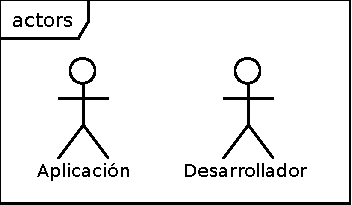
\includegraphics{actors.pdf}\hfill}


\chapter{Requisitos de información}
\label{analysis/ir::doc}\label{analysis/ir:requisitos-de-informacion}

\section{\textbf{IRQ1} Información sobre los usuarios}
\label{analysis/ir:irq1-informacion-sobre-los-usuarios}\begin{itemize}
\item {} 
\textbf{Versión}: 1

\item {} 
\textbf{Autores}: Requisito marcado por la implementación original

\item {} 
\textbf{Fuentes}: Implementación original

\item {} 
\textbf{Objetivos asociados}: OBJ-1, OBJ-3

\item {} 
\textbf{Requisitos asociados}: RF-2, RF-3, RF-4, RF-5, RF-6, RF-7, RF-8

\item {} 
\textbf{Descripción}: La utilidad verifica a través de los diferentes mecanismos de gestión de permisos del sistema los privilegios de cada usuario.

\item {} 
\textbf{Datos específicos}: UID, grupos de usuario

\item {} 
\textbf{Tiempo de vida}: Tiempo de reserva de un Pin

\item {} 
\textbf{Ocurrencias simultáneas}: Tantas como pines se reserven concurrentemente

\item {} 
\textbf{Importancia}: Alta

\item {} 
\textbf{Urgencia}: Alta

\item {} 
\textbf{Estado}: Completo

\item {} 
\textbf{Estabilidad}: Estable

\end{itemize}


\chapter{Requisitos funcionales}
\label{analysis/fr:requisitos-funcionales}\label{analysis/fr::doc}

\section{RF-1: Comunicación con la biblioteca}
\label{analysis/fr:rf-1-comunicacion-con-la-biblioteca}\begin{itemize}
\item {} 
\textbf{Versión}: 1

\item {} 
\textbf{Autores}: Requisito marcado por la implementación original

\item {} 
\textbf{Fuentes}: Implementación original

\item {} 
\textbf{Objetivos asociados}: OBJ-1, OBJ-3

\item {} 
\textbf{Requisitos asociados}: NFR-2

\item {} 
\textbf{Descripción}: Siguiendo el mismo modelo de trabajo de la implementación original, la realización de las diferentes operaciones se realizará mediante llamadas al comando \code{gpio-admin}.

\item {} 
\textbf{Precondición}

\item {} 
\textbf{Secuencia normal}:
\begin{enumerate}
\item {} 
La implementación de la biblioteca solicita la realización de una tarea al comando, especificando los parámetros de la aplicación a través de los parámetros de entrada propios de una llamada al sistema (recogidos en el array \code{argv}).

\item {} 
La biblioteca determina la identidad del usuario mediante el UID del proceso.

\item {} 
Se realiza la operación solicitada y emite un mensaje de confirmación o fallo.

\end{enumerate}

\item {} 
\textbf{Poscondición}: La operación es realizada.

\item {} 
\textbf{Excepciones}:
\begin{itemize}
\item {} 
En el caso de que la biblioteca retorne un error, comienza el caso de uso \textbf{RF-7}

\end{itemize}

\item {} 
\textbf{Rendimiento}: Alto

\item {} 
\textbf{Frecuencia}: Alta

\item {} 
\textbf{Importancia}: Media

\item {} 
\textbf{Urgencia}: Alta

\item {} 
\textbf{Estado}: Completo

\item {} 
\textbf{Estabilidad}: Estable

\end{itemize}


\section{RF-2: ``Registro'' de un pin}
\label{analysis/fr:rf-2-registro-de-un-pin}\begin{itemize}
\item {} 
\textbf{Versión}: 1

\item {} 
\textbf{Autores}: Requisito marcado por la implementación original

\item {} 
\textbf{Fuentes}: Implementación original

\item {} 
\textbf{Objetivos asociados}: OBJ-3

\item {} 
\textbf{Requisitos asociados}: IRQ-1

\item {} 
\textbf{Descripción}: La biblioteca considera que un pin debe ser ``propiedad'' de un usuario antes de poder utilizar el mismo, y a petición de un usuario verificará que el pin solicitado está libre u ocupado, reservándolo en el primer caso.

\item {} 
\textbf{Precondición}

\item {} 
\textbf{Secuencia normal}:
\begin{enumerate}
\item {} 
La aplicación solicita el registro de un pin para su uso a la biblioteca. Comienza el caso de uso RF-1.

\item {} 
Se analiza el código de retorno de la llamada al sistema. En caso de que el pin se encuentre reservado, el caso de uso finaliza y el usuario es notificado. En caso de que el pin no se encuentre reservado, la biblioteca indica que el usuario solicitante es el nuevo propietario.

\item {} 
La biblioteca notifica al usuario de que la reserva ha sido satisfactoria.

\end{enumerate}

\item {} 
\textbf{Poscondición}: El usuario obtiene acceso al pin.

\item {} 
\textbf{Excepciones}: No se plantean excepciones

\item {} 
\textbf{Rendimiento}: Alto

\item {} 
\textbf{Frecuencia}: Generalmente un usuario realizará una reserva en cada ejecución.

\item {} 
\textbf{Importancia}: Alta

\item {} 
\textbf{Urgencia}: Alta

\item {} 
\textbf{Estado}: Completo

\item {} 
\textbf{Estabilidad}: Estable

\end{itemize}


\section{RF-3: ``Liberación'' de un pin}
\label{analysis/fr:rf-3-liberacion-de-un-pin}\begin{itemize}
\item {} 
\textbf{Versión}: 1

\item {} 
\textbf{Autores}: Requisito marcado por la implementación original

\item {} 
\textbf{Fuentes}: Implementación original

\item {} 
\textbf{Objetivos asociados}: OBJ-1, OBJ-3

\item {} 
\textbf{Requisitos asociados}: IRQ-1

\item {} 
\textbf{Descripción}: De la misma forma que un pin es reservado debe ser liberado al finalizar la ejecución, de forma que posteriores usuarios puedan utilizar el mismo.

\item {} 
\textbf{Precondición}: El pin debe estar reservado.

\item {} 
\textbf{Secuencia normal}:
\begin{enumerate}
\item {} 
La aplicación solicita la liberación del pin al comando \code{gpio-admin}. Comienza el caso de uso \emph{RF-1}

\item {} 
La aplicación es notificado del resultado de la operación.

\end{enumerate}

\item {} 
\textbf{Poscondición}: El pin es liberado.

\item {} 
\textbf{Excepciones}: En caso de que se solicite la liberación de un pin no reservado, se notifica a la aplicación y el caso de uso finaliza.

\item {} 
\textbf{Rendimiento}: Alto

\item {} 
\textbf{Frecuencia}: Media

\item {} 
\textbf{Importancia}: Alta

\item {} 
\textbf{Urgencia}: Alta

\item {} 
\textbf{Estado}: Completo

\item {} 
\textbf{Estabilidad}: Estable

\end{itemize}


\section{RF-4: Modificación de la ``dirección'' del pin}
\label{analysis/fr:rf-4-modificacion-de-la-direccion-del-pin}\begin{itemize}
\item {} 
\textbf{Versión}: 1

\item {} 
\textbf{Autores}: Requisito marcado por la implementación original

\item {} 
\textbf{Fuentes}: Implementación original

\item {} 
\textbf{Objetivos asociados}: OBJ-1, OBJ-3

\item {} 
\textbf{Requisitos asociados}: IRQ-1

\item {} 
\textbf{Descripción}: La dirección del pin indica si se utilizará para recibir o enviar información. Todos los pines pueden operar en ambos modos.

\item {} 
\textbf{Precondición}: El pin debe estar reservado previamente.

\item {} 
\textbf{Secuencia normal}:
\begin{enumerate}
\item {} 
La aplicación solicita modificar la dirección del pin al comando \code{gpio-admin}. Comienza el caso de uso \emph{RF-1}.

\end{enumerate}

\item {} 
\textbf{Poscondición}: La dirección del pin es modificada.

\item {} 
\textbf{Excepciones}: En caso de que se solicite la modificación de un pin no reservado, se notifica a la aplicación y el caso de uso finaliza.

\item {} 
\textbf{Rendimiento}

\item {} 
\textbf{Frecuencia}: Se estima que durante cada ejecución se modificará la dirección del pin únicamente durante la fase de inicialización del mismo.

\item {} 
\textbf{Importancia}: Alta

\item {} 
\textbf{Urgencia}: Alta

\item {} 
\textbf{Estado}: Completo

\item {} 
\textbf{Estabilidad}: Estable

\end{itemize}


\section{RF-5: Modificación del valor de un pin}
\label{analysis/fr:rf-5-modificacion-del-valor-de-un-pin}\begin{itemize}
\item {} 
\textbf{Versión}: 1

\item {} 
\textbf{Autores}: Requisito marcado por la implementación original

\item {} 
\textbf{Fuentes}: Implementación original

\item {} 
\textbf{Objetivos asociados}: OBJ-1, OBJ-3

\item {} 
\textbf{Requisitos asociados}: IRQ-1

\item {} 
\textbf{Descripción}: En caso de que la dirección del pin sea de salida, el valor del pin podrá ser modificado (los valores de tensión admitidos con 0 y 5 voltios).

\item {} 
\textbf{Precondición}: El pin debe estar reservado previamente.

\item {} 
\textbf{Secuencia normal}:
\begin{enumerate}
\item {} 
La aplicación solicita modificar el valor del pin al comando \code{gpio-admin}. Comienza el caso de uso \emph{RF-1}.

\end{enumerate}

\item {} 
\textbf{Poscondición}: El valor del pin es modificado.

\item {} 
\textbf{Excepciones}: En caso de que se solicite la modificación de un pin no reservado, se notifica a la aplicación y el caso de uso finaliza.

\item {} 
\textbf{Rendimiento}:

\item {} 
\textbf{Frecuencia}: El número de modificaciones que se realizarán en un programa se estima muy elevado, por lo que el rendimiento deberá ser alto.

\item {} 
\textbf{Importancia}: Alta

\item {} 
\textbf{Urgencia}: Alta

\item {} 
\textbf{Estado}: Completo

\item {} 
\textbf{Estabilidad}: Estable

\end{itemize}


\section{RF-6: Lectura del valor de un pin}
\label{analysis/fr:rf-6-lectura-del-valor-de-un-pin}\begin{itemize}
\item {} 
\textbf{Versión}: 1

\item {} 
\textbf{Autores}: Requisito marcado por la implementación original

\item {} 
\textbf{Fuentes}: Implementación original

\item {} 
\textbf{Objetivos asociados}: OBJ-1, OBJ-3

\item {} 
\textbf{Requisitos asociados}: IRQ-1

\item {} 
\textbf{Descripción}: En caso de que la dirección del pin sea de entrada, el valor (tensión) del pin podrá ser consultado (los valores de trabajo son 0 y 5 voltios).

\item {} 
\textbf{Precondición}: El pin debe estar reservado previamente.

\item {} 
\textbf{Secuencia normal}:
\begin{enumerate}
\item {} 
La aplicación solicita el valor del pin al comando \code{gpio-admin}. Comienza el caso de uso \emph{RF-1}.

\item {} 
Se retorna el valor del pin a la aplicación.

\end{enumerate}

\item {} 
\textbf{Poscondición}: La aplicación cuenta con el valor pin.

\item {} 
\textbf{Excepciones}: En caso de que se solicite la lectura de un pin no reservado, se notifica a la aplicación y el caso de uso finaliza.

\item {} 
\textbf{Rendimiento}:

\item {} 
\textbf{Frecuencia}: El número de consultas que se realizarán en un programa se estima muy elevado, por lo que el rendimiento deberá ser alto.

\item {} 
\textbf{Importancia}: Alta

\item {} 
\textbf{Urgencia}: Alta

\item {} 
\textbf{Estado}: No realizado

\item {} 
\textbf{Estabilidad}: Estable

\end{itemize}


\section{RF-7: Gestión de error}
\label{analysis/fr:rf-7-gestion-de-error}\begin{itemize}
\item {} 
\textbf{Versión}: 1

\item {} 
\textbf{Autores}: Diego Martín

\item {} 
\textbf{Fuentes}: Análisis preliminar

\item {} 
\textbf{Objetivos asociados}: OBJ-1, OBJ-3

\item {} 
\textbf{Requisitos asociados}: NFR-3

\item {} 
\textbf{Descripción}: En el caso de que la biblioteca o la herramienta \code{gpio-admin} retornen un código de error no identificado, comienza este caso de uso.

\item {} 
\textbf{Precondición}: Se debe dar un error en la biblioteca o en \code{gpio-admin}

\item {} 
\textbf{Secuencia normal}:
\begin{enumerate}
\item {} 
La biblioteca intenta identificar el error que se ha dado.

\item {} 
En caso de poder determinarlo envía un mensaje descriptivo a la aplicación. En caso contrario utilizará un mensaje genérico.

\end{enumerate}

\item {} 
\textbf{Poscondición}: La aplicación es informada del error.

\item {} 
\textbf{Excepciones}: No se plantean excepciones

\item {} 
\textbf{Rendimiento}: Medio

\item {} 
\textbf{Frecuencia}: Baja

\item {} 
\textbf{Importancia}: Media

\item {} 
\textbf{Urgencia}: Media

\item {} 
\textbf{Estado}: Completo

\item {} 
\textbf{Estabilidad}: Estable

\end{itemize}


\section{RF-8: Interacción directa con \texttt{gpio-admin}}
\label{analysis/fr:rf-8-interaccion-directa-con-gpio-admin}\begin{itemize}
\item {} 
\textbf{Versión}: 1

\item {} 
\textbf{Autores}: Diego Martín

\item {} 
\textbf{Fuentes}: Análisis preliminar

\item {} 
\textbf{Objetivos asociados}: OBJ-1

\item {} 
\textbf{Requisitos asociados}: IRQ-1

\item {} 
\textbf{Descripción}: La herramienta \code{gpio-admin} puede ser utilizada de forma directa por el usuario, de la misma forma que la biblioteca interactúa con ella.

\item {} 
\textbf{Precondición}: El usuario debe haber iniciado sesión en el sistema.

\item {} 
\textbf{Secuencia normal}:
\begin{enumerate}
\item {} 
El usuario ejecuta la herramienta, utilizando los parámetros de la línea de comandos para indicar la acción a realizar.

\item {} 
La biblioteca ejecuta la acción y muestra los resultados de éxito o error.

\end{enumerate}

\item {} 
\textbf{Poscondición}: La operación a ejecutar se ha llevado a cabo.

\item {} 
\textbf{Excepciones}: En caos de que se dé algún tipo de error, la biblioteca mostrará un mensaje informativo.

\item {} 
\textbf{Rendimiento}: Alto

\item {} 
\textbf{Frecuencia}: Alta

\item {} 
\textbf{Importancia}: Alta

\item {} 
\textbf{Urgencia}: Media

\item {} 
\textbf{Estado}: Completo

\item {} 
\textbf{Estabilidad}: Estable

\end{itemize}


\section{Vista de casos de uso}
\label{analysis/fr:vista-de-casos-de-uso}

\subsection{Vista de paquetes de casos de uso}
\label{analysis/uc::doc}\label{analysis/uc:vista-de-paquetes-de-casos-de-uso}\begin{figure}[htbp]
\centering
\capstart

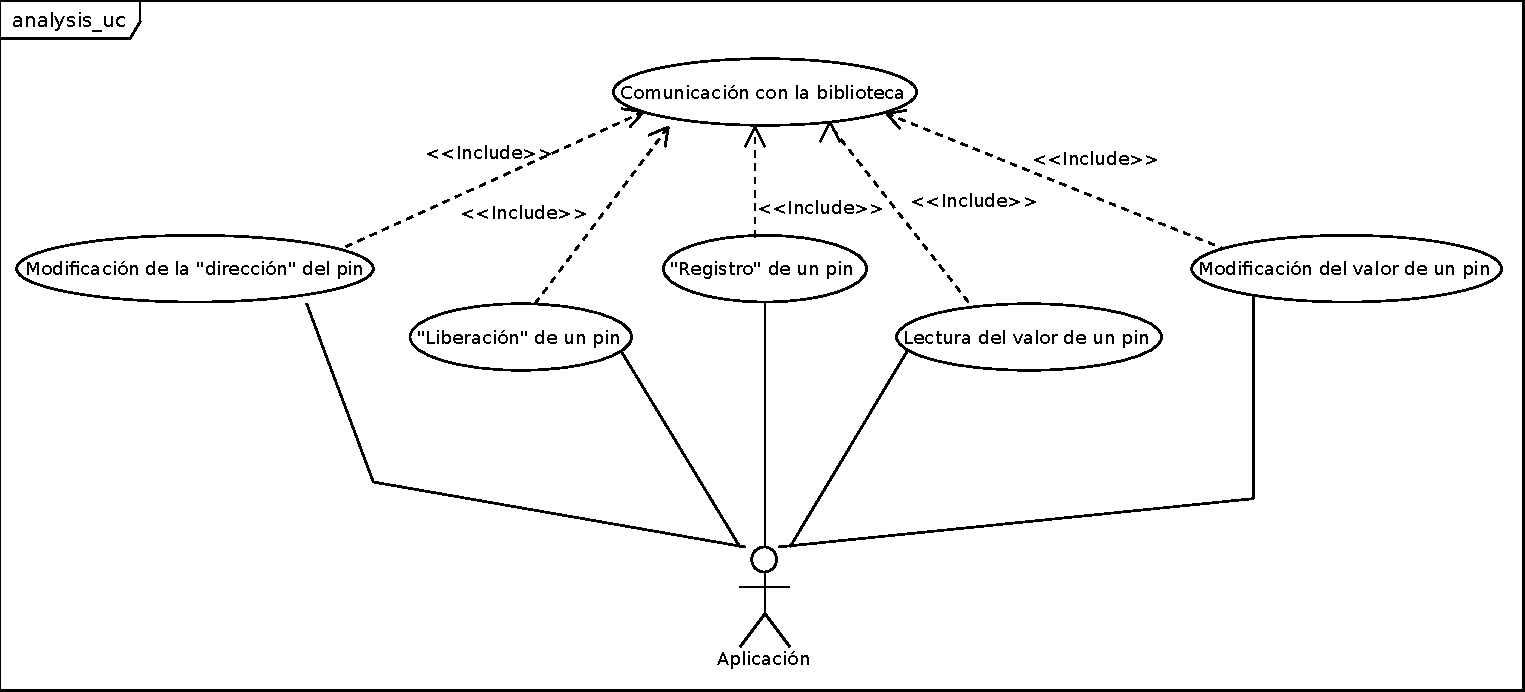
\includegraphics{analysis_uc.pdf}
\caption{Vista del paquete de casos de uso. Se considera que todos los requisitos funcionales son realizados por el actor Aplicación (\textbf{ACT1}), que es implementado por el desarrollador.}\end{figure}


\chapter{Vista de paquetes de casos de uso}
\label{analysis/uc::doc}\label{analysis/uc:vista-de-paquetes-de-casos-de-uso}\begin{figure}[htbp]
\centering
\capstart

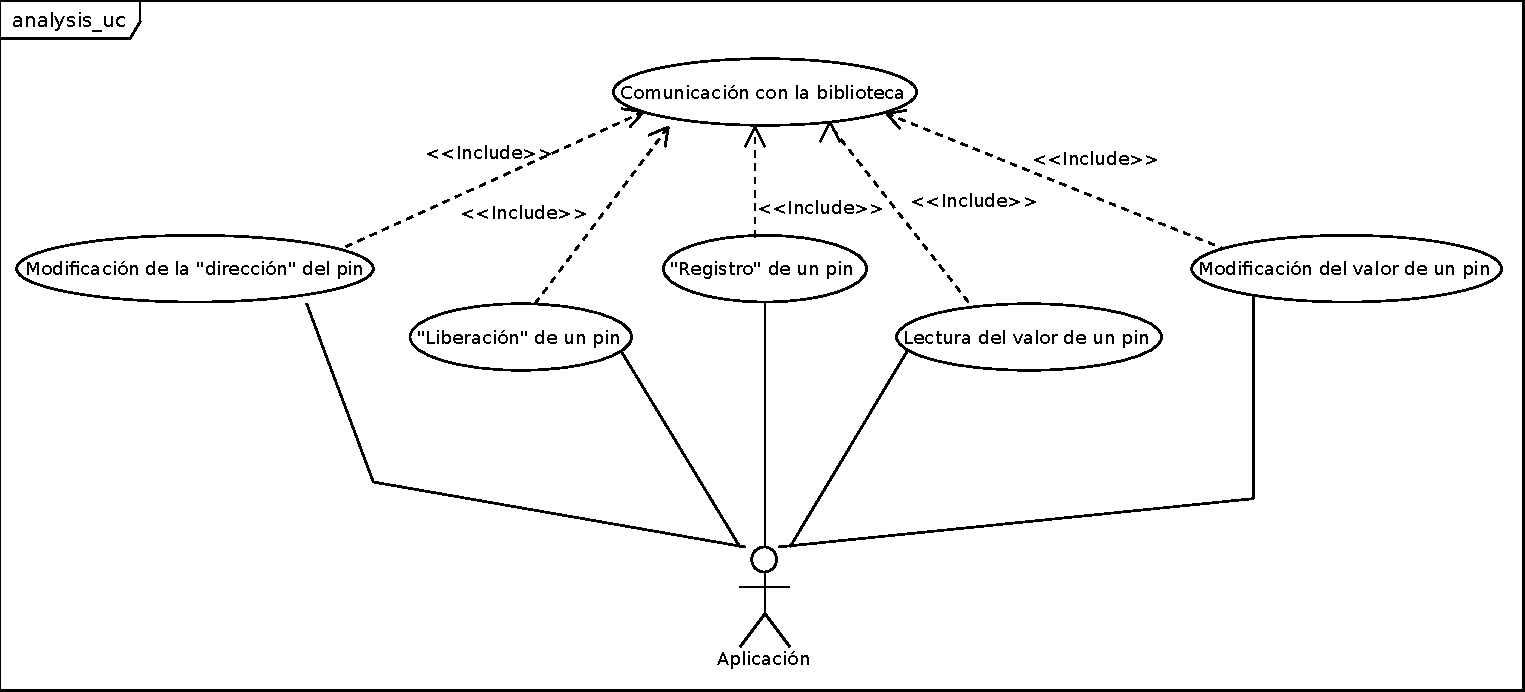
\includegraphics{analysis_uc.pdf}
\caption{Vista del paquete de casos de uso. Se considera que todos los requisitos funcionales son realizados por el actor Aplicación (\textbf{ACT1}), que es implementado por el desarrollador.}\end{figure}


\chapter{Requisitos no funcionales}
\label{analysis/nfr:requisitos-no-funcionales}\label{analysis/nfr::doc}

\section{NFR1: CMake}
\label{analysis/nfr:nfr1-cmake}\begin{itemize}
\item {} 
\textbf{Versión}: 1

\item {} 
\textbf{Autores}: Diego Martín

\item {} 
\textbf{Fuentes}: Análisis preliminar

\item {} 
\textbf{Objetivos asociados}: OBJ-2

\item {} 
\textbf{Descripción}: Se utilizará CMake para la gestión de los diferentes procesos de compilación e instalación del \emph{software}. Además se deberá crear un módulo de CMake que permita localizar la biblioteca creada al ser invocado.

\item {} 
\textbf{Importancia}: Media

\item {} 
\textbf{Urgencia}: Baja

\item {} 
\textbf{Estado}: Completo

\item {} 
\textbf{Estabilidad}: Alta

\end{itemize}


\section{NFR2: Biblioteca compartida}
\label{analysis/nfr:nfr2-biblioteca-compartida}\begin{itemize}
\item {} 
\textbf{Versión}: 1

\item {} 
\textbf{Autores}: Diego Martín

\item {} 
\textbf{Fuentes}: Análisis preliminar

\item {} 
\textbf{Objetivos asociados}: OBJ-2

\item {} 
\textbf{Descripción}: La inclusión de la biblioteca en el sistema debe realizarse en tiempo de ejecución mediante el su compilación como biblioteca compartida.

\item {} 
\textbf{Importancia}: Baja

\item {} 
\textbf{Urgencia}: Baja

\item {} 
\textbf{Estado}: Completo

\item {} 
\textbf{Estabilidad}: Alta

\end{itemize}


\section{NFR3: Similitud}
\label{analysis/nfr:nfr3-similitud}\begin{itemize}
\item {} 
\textbf{Versión}: 1

\item {} 
\textbf{Autores}: Diego Martín

\item {} 
\textbf{Fuentes}: Análisis preliminar

\item {} 
\textbf{Descripción}: A fin de facilitar el trabajo con la API a desarrolladores conocedores de la versión en Python, se conservarán las convenciones de nombres y secuencias de operación que esta utiliza, sin que esto impida aprovechar características de C++ no presentes en Python que se consideren beneficiosas.

\item {} 
\textbf{Importancia}: Media

\item {} 
\textbf{Urgencia}: Media

\item {} 
\textbf{Estado}: Completo

\item {} 
\textbf{Estabilidad}: Estable

\end{itemize}


\section{NFR4: Documentación}
\label{analysis/nfr:nfr4-documentacion}\begin{itemize}
\item {} 
\textbf{Versión}: 1

\item {} 
\textbf{Autores}: Diego Martín

\item {} 
\textbf{Fuentes}: Análisis preliminar

\item {} 
\textbf{Descripción}: La API deberá incluir una documentación fácil de comprender por cualquier desarrollador con conocimientos de C++.

\item {} 
\textbf{Importancia}: Media

\item {} 
\textbf{Urgencia}: Media

\item {} 
\textbf{Estado}: Completo

\item {} 
\textbf{Estabilidad}: Estable

\end{itemize}


\chapter{Vista estática del producto}
\label{analysis/static::doc}\label{analysis/static:vista-estatica-del-producto}\begin{figure}[htbp]
\centering
\capstart

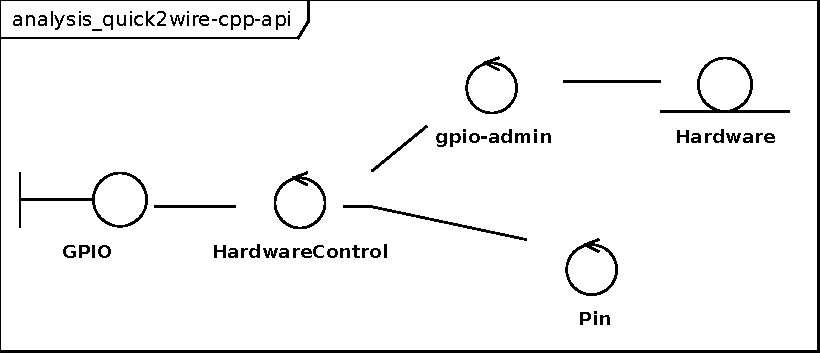
\includegraphics{analysis_quick2wire-cpp-api.pdf}
\caption{La vista estática recoge una clase de interfaz que será aprovechada por las diferentes aplicaciones. Dicha interfaz permitirá el acceso a una clase de control que creará los diferentes objetos de control pin y controlará la comunicación con el comando (interpretado como clase de control) \code{gpio-admin}, que será el encargado de realizar la comunicación con el \emph{hardware}.}\end{figure}


\chapter{Vista de interacción}
\label{analysis/interaction::doc}\label{analysis/interaction:vista-de-interaccion}

\section{Interacción con un pin}
\label{analysis/interaction:interaccion-con-un-pin}\begin{figure}[htbp]
\centering
\capstart

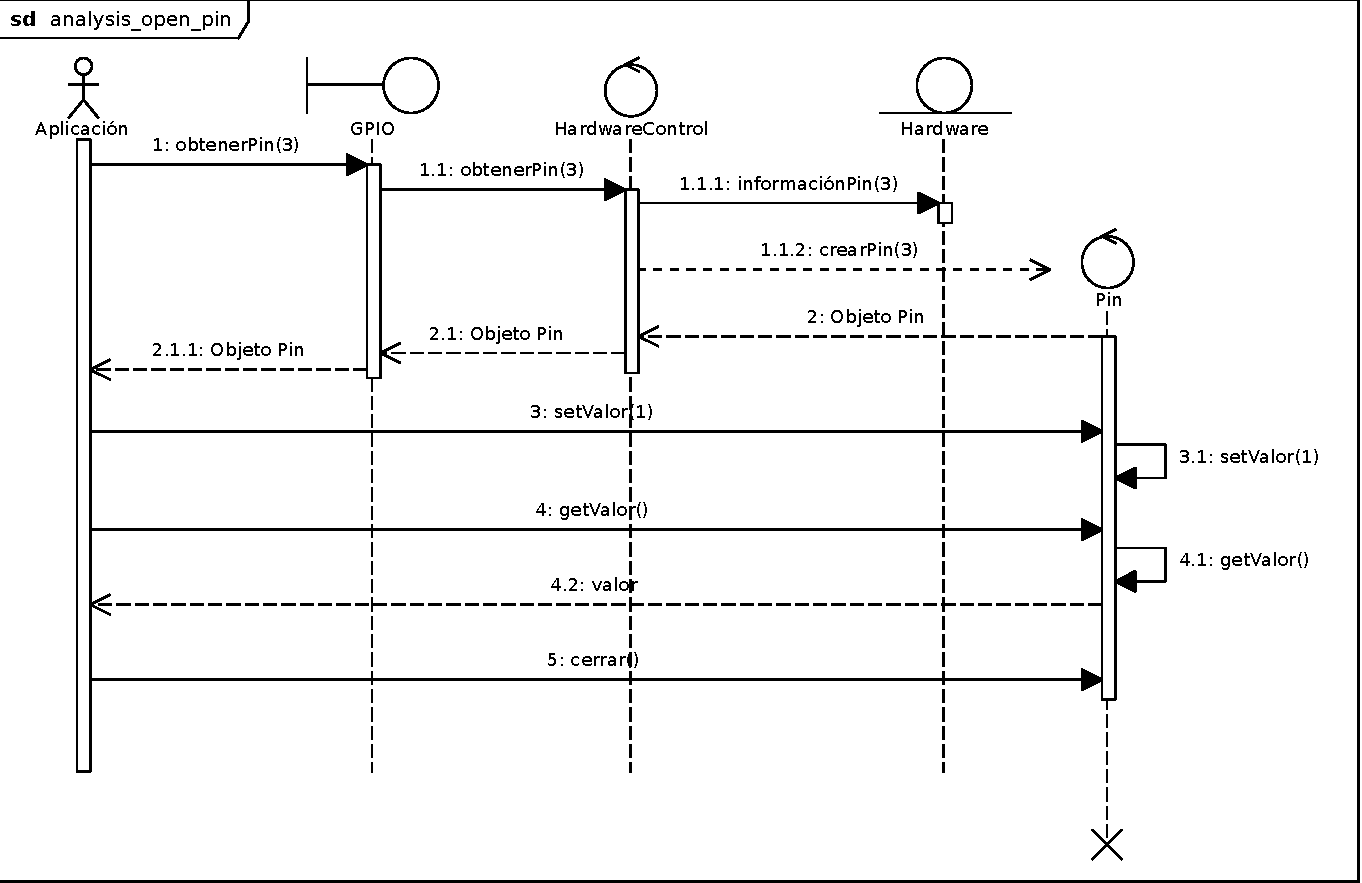
\includegraphics{analysis_open_pin.pdf}
\caption{El diagrama representa un escenario completo de interacción con un pin, desde su reserva hasta la liberación de este.}\end{figure}


\chapter{Vista de máquina de estados}
\label{analysis/states::doc}\label{analysis/states:vista-de-maquina-de-estados}\begin{figure}[htbp]
\centering
\capstart

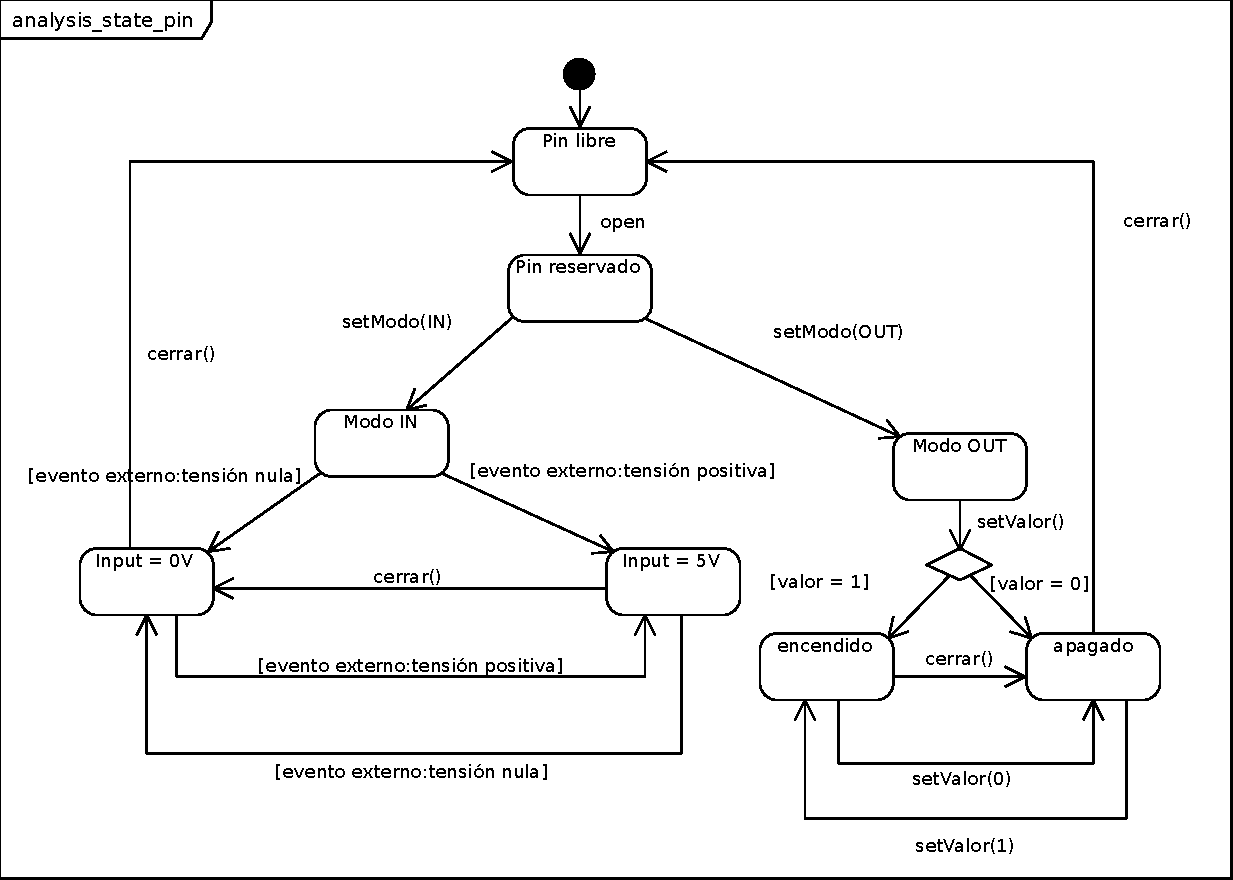
\includegraphics{analysis_state_pin.pdf}
\caption{Representación de todos los estados en los que un pin puede encontrarse. En el caso del modo IN, los eventos que provocan un cambio de estado son provocados por el \emph{hardware} al que el pin se encuentra conectado (por ejemplo, un sensor).}\end{figure}


\chapter{Fase de diseño}
\label{design/intro:fase-de-diseno}\label{design/intro::doc}

\section{Ámbito}
\label{design/scope:ambito}\label{design/scope::doc}
La API se integrará con diferentes aplicaciones mediante su compilación como biblioteca compartida. Este archivo se almacenará en uno de los directorios de búsqueda de bibliotecas del sistema, del mismo modo que los archivos de cabecera serán situados en uno de los directorios de inclusión. La gestión de esta dependencia se ultima con la utilización de un módulo de búsqueda de CMake, por lo que se recomendará su uso (de forma opcional) a los diferentes usuarios.

Los usuarios con privilegios de acceso a la API serán aquellos miembros del grupo \code{gpio}, del cual son miembros todos los desarrolladores de la organización en la que la biblioteca se utilizará.


\section{Diseño de datos}
\label{design/data:diseno-de-datos}\label{design/data::doc}

\subsection{Objetos de datos}
\label{design/data:objetos-de-datos}
Únicamente serán gestionados los objetos pin como contenedores de información, que permitirán consultar la información del pin al que apuntan.


\subsection{Estructuras de archivo}
\label{design/data:estructuras-de-archivo}
Se consultarán los grupos de los que un usuario es miembro, generalmente recogidos en el fichero \code{/etc/passwd}.


\section{Diseño arquitectónico}
\label{design/architecture::doc}\label{design/architecture:diseno-arquitectonico}
{\hfill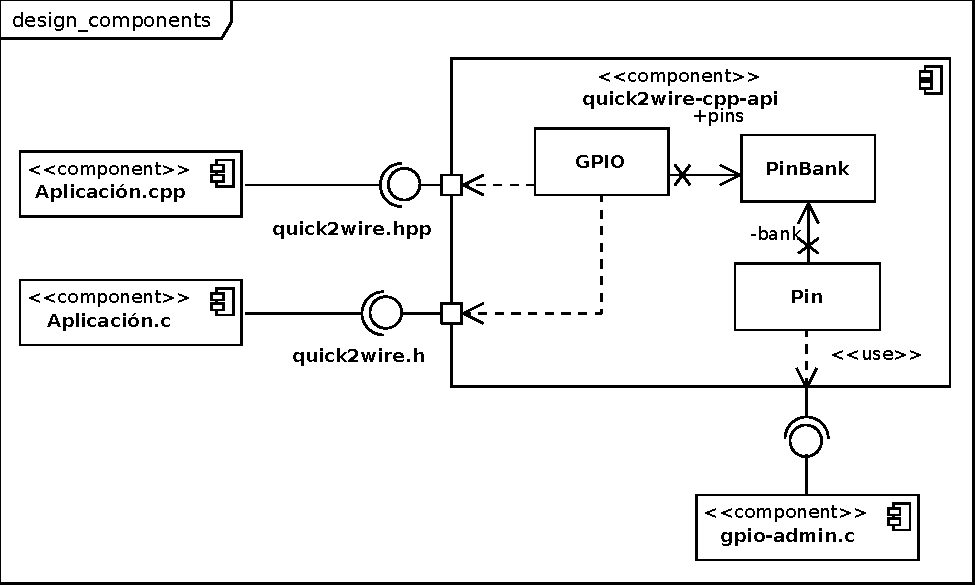
\includegraphics{design_components.pdf}\hfill}


\section{Despliegue}
\label{design/deployment::doc}\label{design/deployment:despliegue}\begin{figure}[htbp]
\centering
\capstart

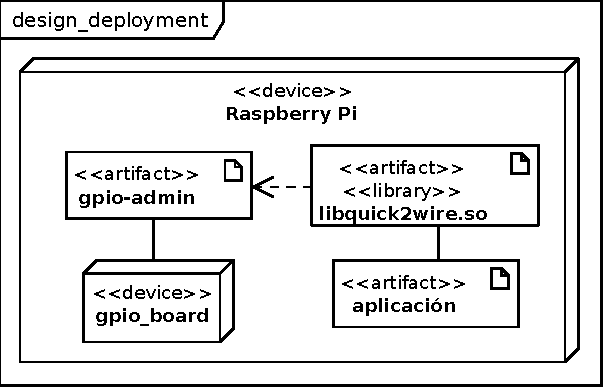
\includegraphics{design_deployment.pdf}
\caption{Representación de los diferentes componentes y sus interacciones. Nótese que el hardware GPIO se representa como componente del dispositivo Raspberry Pi}\end{figure}


\section{Vista estática del producto}
\label{design/static::doc}\label{design/static:vista-estatica-del-producto}

\subsection{API}
\label{design/static:api}\begin{figure}[htbp]
\centering
\capstart

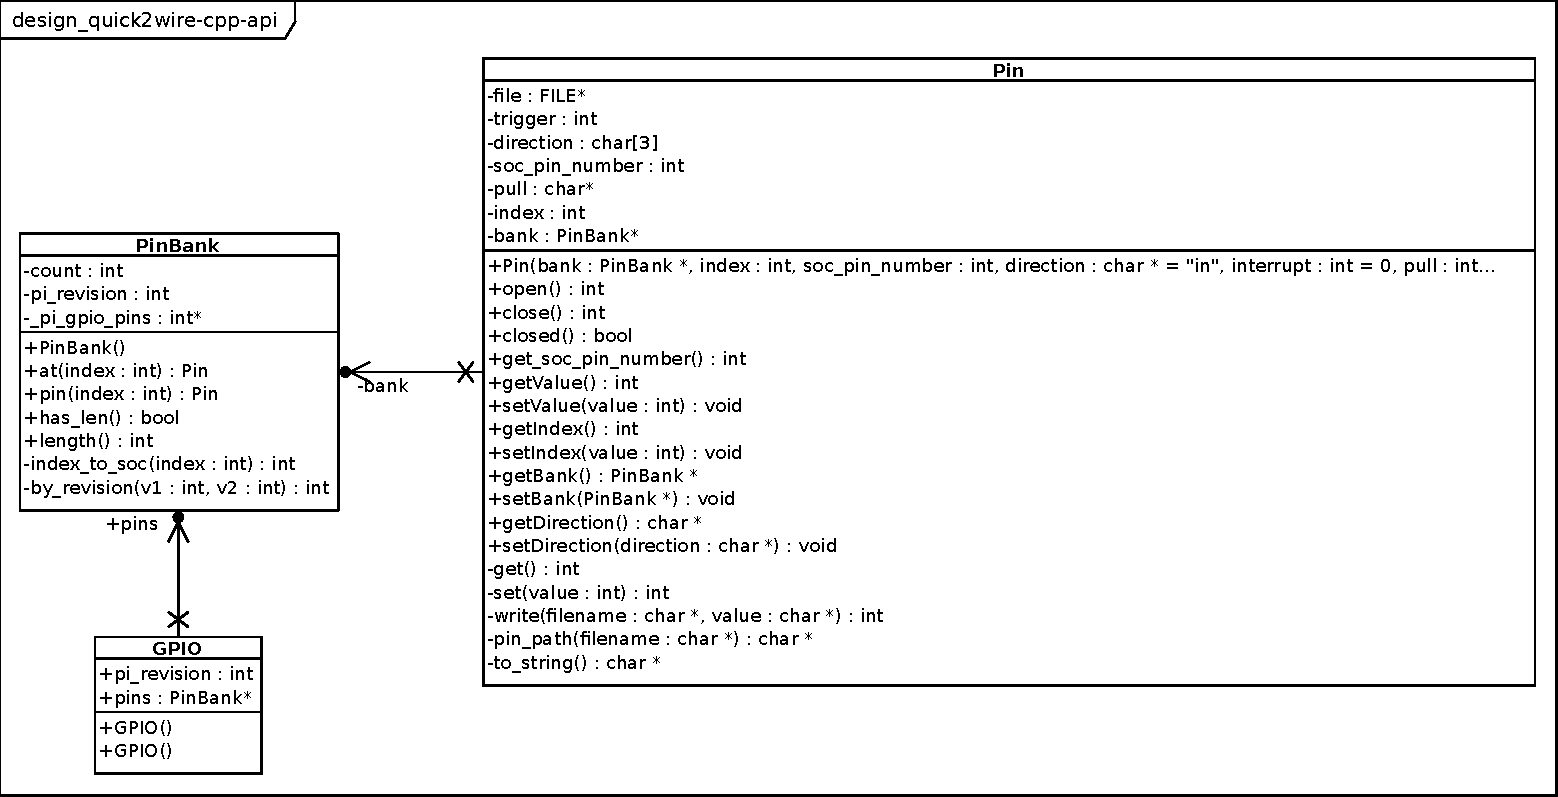
\includegraphics{design_quick2wire-cpp-api.pdf}
\caption{La API utiliza como punto de entrada la clase \code{GPIO}, que gestionará un objeto \code{PinBank}, el cual se encargará de la gestión de los diferentes pines.}\end{figure}


\subsection{gpio-admin}
\label{design/static:gpio-admin}\begin{figure}[htbp]
\centering
\capstart

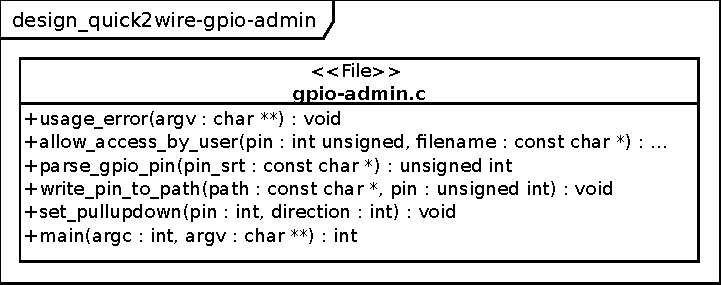
\includegraphics{design_quick2wire-gpio-admin.pdf}
\caption{El ejecutable \code{gpio-admin} no se implementa siguiendo el paradigma de orientación a objetos. Se representa en el diagrama mediante una clase con el estereotipo \code{\textless{}\textless{}file\textgreater{}\textgreater{}}.}\end{figure}


\section{Diseño procedimental}
\label{design/procedimental:diseno-procedimental}\label{design/procedimental::doc}
En este apartado se referencian los algoritmos implementados en el sistema que son considerados de mayor relevancia.

Detección de la versión de la placa, para adaptar el número de pines ofrecidos al valor físico.

\begin{Verbatim}[commandchars=\\\{\}]
\PYG{c+cp}{\PYGZsh{}}\PYG{c+cp}{include \PYGZdq{}board\PYGZus{}revision.hpp\PYGZdq{}}

\PYG{c+cp}{\PYGZsh{}}\PYG{c+cp}{define CPUINFO\PYGZus{}PATH \PYGZdq{}}\PYG{c+cp}{/}\PYG{c+cp}{proc}\PYG{c+cp}{/}\PYG{c+cp}{cpuinfo\PYGZdq{}}

\PYG{c+cp}{\PYGZsh{}}\PYG{c+cp}{define PI\PYGZus{}VERSION\PYGZus{}1 1}
\PYG{c+cp}{\PYGZsh{}}\PYG{c+cp}{define PI\PYGZus{}VERSION\PYGZus{}2 2}
\PYG{k+kt}{int} \PYG{n+nf}{revision}\PYG{p}{(}\PYG{p}{)}\PYG{p}{\PYGZob{}}
	\PYG{n}{std}\PYG{o}{:}\PYG{o}{:}\PYG{n}{ifstream} \PYG{n}{fcpuinfo}\PYG{p}{(}\PYG{n}{CPUINFO\PYGZus{}PATH}\PYG{p}{)}\PYG{p}{;}
	\PYG{k}{if}\PYG{p}{(}\PYG{n}{fcpuinfo}\PYG{p}{.}\PYG{n}{fail}\PYG{p}{(}\PYG{p}{)}\PYG{p}{)}\PYG{p}{\PYGZob{}}
		\PYG{k}{return} \PYG{l+m+mi}{3}\PYG{p}{;}
	\PYG{p}{\PYGZcb{}}
	\PYG{n}{std}\PYG{o}{:}\PYG{o}{:}\PYG{n}{string} \PYG{n}{aux\PYGZus{}str}\PYG{p}{;}
	\PYG{n}{std}\PYG{o}{:}\PYG{o}{:}\PYG{n}{string} \PYG{n}{revision\PYGZus{}str}\PYG{p}{(}\PYG{l+s}{\PYGZdq{}}\PYG{l+s}{Revision}\PYG{l+s}{\PYGZdq{}}\PYG{p}{)}\PYG{p}{;}
	\PYG{k}{while}\PYG{p}{(}\PYG{n}{std}\PYG{o}{:}\PYG{o}{:}\PYG{n}{getline}\PYG{p}{(}\PYG{n}{fcpuinfo}\PYG{p}{,} \PYG{n}{aux\PYGZus{}str}\PYG{p}{)}\PYG{p}{)}\PYG{p}{\PYGZob{}}
		\PYG{k}{if}\PYG{p}{(}\PYG{n}{revision\PYGZus{}str}\PYG{p}{.}\PYG{n}{compare}\PYG{p}{(}\PYG{l+m+mi}{0}\PYG{p}{,} \PYG{n}{revision\PYGZus{}str}\PYG{p}{.}\PYG{n}{length}\PYG{p}{(}\PYG{p}{)}\PYG{p}{,} \PYG{n}{aux\PYGZus{}str}\PYG{p}{.}\PYG{n}{substr}\PYG{p}{(}\PYG{l+m+mi}{0}\PYG{p}{,} \PYG{n}{revision\PYGZus{}str}\PYG{p}{.}\PYG{n}{length}\PYG{p}{(}\PYG{p}{)}\PYG{p}{)}\PYG{p}{)} \PYG{o}{=}\PYG{o}{=} \PYG{l+m+mi}{0}\PYG{p}{)}\PYG{p}{\PYGZob{}}
			\PYG{k}{if}\PYG{p}{(}\PYG{p}{(}\PYG{n}{aux\PYGZus{}str}\PYG{p}{.}\PYG{n}{compare}\PYG{p}{(}\PYG{n}{aux\PYGZus{}str}\PYG{p}{.}\PYG{n}{length}\PYG{p}{(}\PYG{p}{)} \PYG{o}{\PYGZhy{}} \PYG{l+m+mi}{2}\PYG{p}{,} \PYG{n}{aux\PYGZus{}str}\PYG{p}{.}\PYG{n}{length}\PYG{p}{(}\PYG{p}{)} \PYG{o}{\PYGZhy{}}\PYG{l+m+mi}{1}\PYG{p}{,} \PYG{l+s}{\PYGZdq{}}\PYG{l+s}{2}\PYG{l+s}{\PYGZdq{}}\PYG{p}{)} \PYG{o}{=}\PYG{o}{=} \PYG{l+m+mi}{0}\PYG{p}{)} \PYG{o}{\textbar{}}\PYG{o}{\textbar{}} \PYG{p}{(}\PYG{n}{aux\PYGZus{}str}\PYG{p}{.}\PYG{n}{compare}\PYG{p}{(}\PYG{n}{aux\PYGZus{}str}\PYG{p}{.}\PYG{n}{length}\PYG{p}{(}\PYG{p}{)} \PYG{o}{\PYGZhy{}} \PYG{l+m+mi}{2}\PYG{p}{,} \PYG{n}{aux\PYGZus{}str}\PYG{p}{.}\PYG{n}{length}\PYG{p}{(}\PYG{p}{)} \PYG{o}{\PYGZhy{}} \PYG{l+m+mi}{1}\PYG{p}{,} \PYG{l+s}{\PYGZdq{}}\PYG{l+s}{3}\PYG{l+s}{\PYGZdq{}}\PYG{p}{)} \PYG{o}{=}\PYG{o}{=} \PYG{l+m+mi}{0}\PYG{p}{)}\PYG{p}{)}\PYG{p}{\PYGZob{}}
				\PYG{k}{return} \PYG{l+m+mi}{1}\PYG{p}{;}
			\PYG{p}{\PYGZcb{}}
			\PYG{k}{return} \PYG{l+m+mi}{2}\PYG{p}{;}
		\PYG{p}{\PYGZcb{}}
	\PYG{p}{\PYGZcb{}}
	\PYG{k}{return} \PYG{l+m+mi}{0}\PYG{p}{;}
\PYG{p}{\PYGZcb{}}
\end{Verbatim}

Apertura de un pin mediante una llamada al comando \code{gpio-admin}.

\begin{Verbatim}[commandchars=\\\{\}]
\PYG{k+kt}{int} \PYG{n+nf}{gpio\PYGZus{}admin}\PYG{p}{(}\PYG{k+kt}{char} \PYG{o}{*} \PYG{n}{subcommand}\PYG{p}{,} \PYG{k+kt}{int} \PYG{n}{pin}\PYG{p}{,} \PYG{k+kt}{char}\PYG{o}{*} \PYG{n}{pull}\PYG{p}{)}\PYG{p}{\PYGZob{}}

	\PYG{k+kt}{char} \PYG{n}{command}\PYG{p}{[}\PYG{n}{MAX\PYGZus{}LEN}\PYG{p}{]}\PYG{p}{;}
	
	\PYG{n}{snprintf}\PYG{p}{(}\PYG{n}{command}\PYG{p}{,} \PYG{n}{MAX\PYGZus{}LEN}\PYG{p}{,} \PYG{l+s}{\PYGZdq{}}\PYG{l+s}{gpio\PYGZhy{}admin \PYGZpc{}s \PYGZpc{}d}\PYG{l+s+se}{\PYGZbs{}n}\PYG{l+s}{\PYGZdq{}}\PYG{p}{,} \PYG{n}{subcommand}\PYG{p}{,} \PYG{n}{pin}\PYG{p}{)}\PYG{p}{;}\PYG{c+c1}{//, pull == NULL ? \PYGZdq{}\PYGZdq{} : pull);}
	\PYG{k+kt}{FILE}\PYG{o}{*} \PYG{n}{f} \PYG{o}{=} \PYG{n}{popen}\PYG{p}{(}\PYG{n}{command}\PYG{p}{,} \PYG{l+s}{\PYGZdq{}}\PYG{l+s}{r}\PYG{l+s}{\PYGZdq{}}\PYG{p}{)}\PYG{p}{;}
	
	\PYG{k}{return} \PYG{n}{pclose}\PYG{p}{(}\PYG{n}{f}\PYG{p}{)}\PYG{p}{;}
\PYG{p}{\PYGZcb{}}
\PYG{k+kt}{int} \PYG{n}{Pin}\PYG{o}{:}\PYG{o}{:}\PYG{n}{open}\PYG{p}{(}\PYG{p}{)}\PYG{p}{\PYGZob{}}
 	\PYG{n}{gpio\PYGZus{}admin}\PYG{p}{(}\PYG{l+s}{\PYGZdq{}}\PYG{l+s}{export}\PYG{l+s}{\PYGZdq{}}\PYG{p}{,} \PYG{n}{this}\PYG{o}{\PYGZhy{}}\PYG{o}{\PYGZgt{}}\PYG{n}{soc\PYGZus{}pin\PYGZus{}number}\PYG{p}{,} \PYG{n}{this}\PYG{o}{\PYGZhy{}}\PYG{o}{\PYGZgt{}}\PYG{n}{pull}\PYG{p}{)}\PYG{p}{;}
 	\PYG{k}{if}\PYG{p}{(}\PYG{n+nb}{NULL} \PYG{o}{=}\PYG{o}{=} \PYG{p}{(}\PYG{n}{this}\PYG{o}{\PYGZhy{}}\PYG{o}{\PYGZgt{}}\PYG{n}{file} \PYG{o}{=} \PYG{n}{fopen}\PYG{p}{(}\PYG{n}{this}\PYG{o}{\PYGZhy{}}\PYG{o}{\PYGZgt{}}\PYG{n}{pin\PYGZus{}path}\PYG{p}{(}\PYG{l+s}{\PYGZdq{}}\PYG{l+s}{value}\PYG{l+s}{\PYGZdq{}}\PYG{p}{)}\PYG{p}{,} \PYG{l+s}{\PYGZdq{}}\PYG{l+s}{r+}\PYG{l+s}{\PYGZdq{}}\PYG{p}{)}\PYG{p}{)}\PYG{p}{)}\PYG{p}{\PYGZob{}}
 		\PYG{n}{quick2wire\PYGZus{}errno} \PYG{o}{=} \PYG{n}{PIN\PYGZus{}ERR}\PYG{p}{;}
 		\PYG{k}{return} \PYG{l+m+mi}{1}\PYG{p}{;}
	\PYG{p}{\PYGZcb{}}
	
 	\PYG{k}{return} \PYG{n}{this}\PYG{o}{\PYGZhy{}}\PYG{o}{\PYGZgt{}}\PYG{n}{write}\PYG{p}{(}\PYG{l+s}{\PYGZdq{}}\PYG{l+s}{direction}\PYG{l+s}{\PYGZdq{}}\PYG{p}{,} \PYG{n}{this}\PYG{o}{\PYGZhy{}}\PYG{o}{\PYGZgt{}}\PYG{n}{direction}\PYG{p}{)}\PYG{p}{;}

	\PYG{c+cm}{/*if self.\PYGZus{}direction == In:}
\PYG{c+cm}{        self.\PYGZus{}write(\PYGZdq{}edge\PYGZdq{}, self.\PYGZus{}interrupt if self.\PYGZus{}interrupt is not None else \PYGZdq{}none\PYGZdq{})}
\PYG{c+cm}{    */}
\PYG{p}{\PYGZcb{}}
\end{Verbatim}

Modificación del valor de un pin.

\begin{Verbatim}[commandchars=\\\{\}]
\PYG{k+kt}{int} \PYG{n}{Pin}\PYG{o}{:}\PYG{o}{:}\PYG{n}{set}\PYG{p}{(}\PYG{k+kt}{int} \PYG{n}{value}\PYG{p}{)}\PYG{p}{\PYGZob{}}
	
	\PYG{k}{if}\PYG{p}{(}\PYG{n}{this}\PYG{o}{\PYGZhy{}}\PYG{o}{\PYGZgt{}}\PYG{n}{closed}\PYG{p}{(}\PYG{p}{)}\PYG{p}{)}\PYG{p}{\PYGZob{}}
		\PYG{n}{perror}\PYG{p}{(}\PYG{l+s}{\PYGZdq{}}\PYG{l+s}{The device is closed}\PYG{l+s}{\PYGZdq{}}\PYG{p}{)}\PYG{p}{;}
		\PYG{k}{return} \PYG{o}{\PYGZhy{}}\PYG{l+m+mi}{1}\PYG{p}{;}
	\PYG{p}{\PYGZcb{}}
	\PYG{k}{if}\PYG{p}{(}\PYG{n}{strcmp}\PYG{p}{(}\PYG{n}{OUT}\PYG{p}{,} \PYG{l+s}{\PYGZdq{}}\PYG{l+s}{out}\PYG{l+s}{\PYGZdq{}}\PYG{p}{)} \PYG{o}{!}\PYG{o}{=} \PYG{l+m+mi}{0}\PYG{p}{)}\PYG{p}{\PYGZob{}}
		\PYG{n}{perror}\PYG{p}{(}\PYG{l+s}{\PYGZdq{}}\PYG{l+s}{The direction is not }\PYG{l+s+se}{\PYGZbs{}\PYGZdq{}}\PYG{l+s}{out}\PYG{l+s+se}{\PYGZbs{}\PYGZdq{}}\PYG{l+s}{\PYGZdq{}}\PYG{p}{)}\PYG{p}{;}
		\PYG{k}{return} \PYG{o}{\PYGZhy{}}\PYG{l+m+mi}{2}\PYG{p}{;}
	\PYG{p}{\PYGZcb{}}
	
	\PYG{n}{fseek}\PYG{p}{(}\PYG{n}{this}\PYG{o}{\PYGZhy{}}\PYG{o}{\PYGZgt{}}\PYG{n}{file}\PYG{p}{,} \PYG{l+m+mi}{0}\PYG{p}{,} \PYG{n}{SEEK\PYGZus{}SET}\PYG{p}{)}\PYG{p}{;}
	
	\PYG{k+kt}{char} \PYG{n}{buff}\PYG{p}{[}\PYG{l+m+mi}{3}\PYG{p}{]}\PYG{p}{;}
	\PYG{n}{snprintf}\PYG{p}{(}\PYG{n}{buff}\PYG{p}{,} \PYG{l+m+mi}{3}\PYG{p}{,} \PYG{l+s}{\PYGZdq{}}\PYG{l+s}{\PYGZpc{}d}\PYG{l+s}{\PYGZdq{}}\PYG{p}{,} \PYG{n}{value}\PYG{p}{)}\PYG{p}{;}
	\PYG{n}{fputs}\PYG{p}{(}\PYG{n}{buff}\PYG{p}{,} \PYG{n}{this}\PYG{o}{\PYGZhy{}}\PYG{o}{\PYGZgt{}}\PYG{n}{file}\PYG{p}{)}\PYG{p}{;}
	\PYG{n}{fflush}\PYG{p}{(}\PYG{n}{this}\PYG{o}{\PYGZhy{}}\PYG{o}{\PYGZgt{}}\PYG{n}{file}\PYG{p}{)}\PYG{p}{;}
	
	\PYG{k}{return} \PYG{n}{value}\PYG{p}{;}
\PYG{p}{\PYGZcb{}}
\end{Verbatim}


\section{Pruebas}
\label{design/tests::doc}\label{design/tests:pruebas}
Se han realizado pruebas de concepto para el uso de la biblioteca (ver la sección ``Examples'' de la documentación técnica). Además de pruebas unitarias manuales y pruebas de integración con aplicaciones ya creadas o programadas explícitamente con el fin de probar la biblioteca, integrando la misma con la biblioteca MPI.


\chapter{Gestión del proyecto}
\label{project_mgmt/intro:gestion-del-proyecto}\label{project_mgmt/intro::doc}
La gestión del proyecto comienza en la iteración número 10 (issue \#101 en Redmine), realizando una etapa de análisis previa para determinar la viabilidad de diferentes alternativas. Todas las tareas de desarrollo terminan en dicha iteración, añadiéndose varias tareas en la iteración número 13 (issue \#148 en Redmine) relacionadas con nuevas características u operaciones de soporte.


\chapter{Indices and tables}
\label{index:indices-and-tables}\begin{itemize}
\item {} 
\DUspan{xref,std,std-ref}{genindex}

\item {} 
\DUspan{xref,std,std-ref}{modindex}

\item {} 
\DUspan{xref,std,std-ref}{search}

\end{itemize}



\renewcommand{\indexname}{Índice}
\printindex
\end{document}
